% Options for packages loaded elsewhere
\PassOptionsToPackage{unicode}{hyperref}
\PassOptionsToPackage{hyphens}{url}
%
\documentclass[
  english,
  man]{apa6}
\usepackage{amsmath,amssymb}
\usepackage{lmodern}
\usepackage{ifxetex,ifluatex}
\ifnum 0\ifxetex 1\fi\ifluatex 1\fi=0 % if pdftex
  \usepackage[T1]{fontenc}
  \usepackage[utf8]{inputenc}
  \usepackage{textcomp} % provide euro and other symbols
\else % if luatex or xetex
  \usepackage{unicode-math}
  \defaultfontfeatures{Scale=MatchLowercase}
  \defaultfontfeatures[\rmfamily]{Ligatures=TeX,Scale=1}
\fi
% Use upquote if available, for straight quotes in verbatim environments
\IfFileExists{upquote.sty}{\usepackage{upquote}}{}
\IfFileExists{microtype.sty}{% use microtype if available
  \usepackage[]{microtype}
  \UseMicrotypeSet[protrusion]{basicmath} % disable protrusion for tt fonts
}{}
\makeatletter
\@ifundefined{KOMAClassName}{% if non-KOMA class
  \IfFileExists{parskip.sty}{%
    \usepackage{parskip}
  }{% else
    \setlength{\parindent}{0pt}
    \setlength{\parskip}{6pt plus 2pt minus 1pt}}
}{% if KOMA class
  \KOMAoptions{parskip=half}}
\makeatother
\usepackage{xcolor}
\IfFileExists{xurl.sty}{\usepackage{xurl}}{} % add URL line breaks if available
\IfFileExists{bookmark.sty}{\usepackage{bookmark}}{\usepackage{hyperref}}
\hypersetup{
  pdftitle={Detecting Hate speech using Natural Language processing},
  pdfauthor={Vinita V. Vader1},
  pdflang={en-EN},
  pdfkeywords={Hate speech, NLP, RoBERTa},
  hidelinks,
  pdfcreator={LaTeX via pandoc}}
\urlstyle{same} % disable monospaced font for URLs
\usepackage{graphicx}
\makeatletter
\def\maxwidth{\ifdim\Gin@nat@width>\linewidth\linewidth\else\Gin@nat@width\fi}
\def\maxheight{\ifdim\Gin@nat@height>\textheight\textheight\else\Gin@nat@height\fi}
\makeatother
% Scale images if necessary, so that they will not overflow the page
% margins by default, and it is still possible to overwrite the defaults
% using explicit options in \includegraphics[width, height, ...]{}
\setkeys{Gin}{width=\maxwidth,height=\maxheight,keepaspectratio}
% Set default figure placement to htbp
\makeatletter
\def\fps@figure{htbp}
\makeatother
\setlength{\emergencystretch}{3em} % prevent overfull lines
\providecommand{\tightlist}{%
  \setlength{\itemsep}{0pt}\setlength{\parskip}{0pt}}
\setcounter{secnumdepth}{-\maxdimen} % remove section numbering
% Make \paragraph and \subparagraph free-standing
\ifx\paragraph\undefined\else
  \let\oldparagraph\paragraph
  \renewcommand{\paragraph}[1]{\oldparagraph{#1}\mbox{}}
\fi
\ifx\subparagraph\undefined\else
  \let\oldsubparagraph\subparagraph
  \renewcommand{\subparagraph}[1]{\oldsubparagraph{#1}\mbox{}}
\fi
% Manuscript styling
\usepackage{upgreek}
\captionsetup{font=singlespacing,justification=justified}

% Table formatting
\usepackage{longtable}
\usepackage{lscape}
% \usepackage[counterclockwise]{rotating}   % Landscape page setup for large tables
\usepackage{multirow}		% Table styling
\usepackage{tabularx}		% Control Column width
\usepackage[flushleft]{threeparttable}	% Allows for three part tables with a specified notes section
\usepackage{threeparttablex}            % Lets threeparttable work with longtable

% Create new environments so endfloat can handle them
% \newenvironment{ltable}
%   {\begin{landscape}\centering\begin{threeparttable}}
%   {\end{threeparttable}\end{landscape}}
\newenvironment{lltable}{\begin{landscape}\centering\begin{ThreePartTable}}{\end{ThreePartTable}\end{landscape}}

% Enables adjusting longtable caption width to table width
% Solution found at http://golatex.de/longtable-mit-caption-so-breit-wie-die-tabelle-t15767.html
\makeatletter
\newcommand\LastLTentrywidth{1em}
\newlength\longtablewidth
\setlength{\longtablewidth}{1in}
\newcommand{\getlongtablewidth}{\begingroup \ifcsname LT@\roman{LT@tables}\endcsname \global\longtablewidth=0pt \renewcommand{\LT@entry}[2]{\global\advance\longtablewidth by ##2\relax\gdef\LastLTentrywidth{##2}}\@nameuse{LT@\roman{LT@tables}} \fi \endgroup}

% \setlength{\parindent}{0.5in}
% \setlength{\parskip}{0pt plus 0pt minus 0pt}

% \usepackage{etoolbox}
\makeatletter
\patchcmd{\HyOrg@maketitle}
  {\section{\normalfont\normalsize\abstractname}}
  {\section*{\normalfont\normalsize\abstractname}}
  {}{\typeout{Failed to patch abstract.}}
\patchcmd{\HyOrg@maketitle}
  {\section{\protect\normalfont{\@title}}}
  {\section*{\protect\normalfont{\@title}}}
  {}{\typeout{Failed to patch title.}}
\makeatother
\shorttitle{Hate speech Detection}
\keywords{Hate speech, NLP, RoBERTa\newline\indent Word count: X}
\DeclareDelayedFloatFlavor{ThreePartTable}{table}
\DeclareDelayedFloatFlavor{lltable}{table}
\DeclareDelayedFloatFlavor*{longtable}{table}
\makeatletter
\renewcommand{\efloat@iwrite}[1]{\immediate\expandafter\protected@write\csname efloat@post#1\endcsname{}}
\makeatother
\usepackage{lineno}

\linenumbers
\usepackage{csquotes}
\usepackage{setspace}
\AtBeginEnvironment{tabular}{\singlespacing}
\AtBeginEnvironment{lltable}{\singlespacing}
\AtBeginEnvironment{tablenotes}{\doublespacing}
\captionsetup[table]{font={stretch=1.5}}
\captionsetup[figure]{font={stretch=1.5}}
\ifxetex
  % Load polyglossia as late as possible: uses bidi with RTL langages (e.g. Hebrew, Arabic)
  \usepackage{polyglossia}
  \setmainlanguage[]{english}
\else
  \usepackage[main=english]{babel}
% get rid of language-specific shorthands (see #6817):
\let\LanguageShortHands\languageshorthands
\def\languageshorthands#1{}
\fi
\ifluatex
  \usepackage{selnolig}  % disable illegal ligatures
\fi
\newlength{\cslhangindent}
\setlength{\cslhangindent}{1.5em}
\newlength{\csllabelwidth}
\setlength{\csllabelwidth}{3em}
\newenvironment{CSLReferences}[2] % #1 hanging-ident, #2 entry spacing
 {% don't indent paragraphs
  \setlength{\parindent}{0pt}
  % turn on hanging indent if param 1 is 1
  \ifodd #1 \everypar{\setlength{\hangindent}{\cslhangindent}}\ignorespaces\fi
  % set entry spacing
  \ifnum #2 > 0
  \setlength{\parskip}{#2\baselineskip}
  \fi
 }%
 {}
\usepackage{calc}
\newcommand{\CSLBlock}[1]{#1\hfill\break}
\newcommand{\CSLLeftMargin}[1]{\parbox[t]{\csllabelwidth}{#1}}
\newcommand{\CSLRightInline}[1]{\parbox[t]{\linewidth - \csllabelwidth}{#1}\break}
\newcommand{\CSLIndent}[1]{\hspace{\cslhangindent}#1}

\title{Detecting Hate speech using Natural Language processing}
\author{Vinita V. Vader\textsuperscript{1}}
\date{}


\authornote{

Vinita V.Vader, University of Oregon, Department of Psychology, 1227 University of Oregon, Eugene, OR, 97403

Correspondence concerning this article should be addressed to Vinita V. Vader, Department of Psychology, 1227 University of Oregon, Eugene, OR, 97403. E-mail: \href{mailto:vvader@uoregon.edu}{\nolinkurl{vvader@uoregon.edu}}

}

\affiliation{\vspace{0.5cm}\textsuperscript{1} University of Oregon}

\begin{document}
\maketitle

\hypertarget{research-problem}{%
\section{Research problem}\label{research-problem}}

\begin{quote}
Describe the task you want to achieve. What is the outcome of interest? What are you trying to predict? Why is it important? What are the potential benefits of having a predictive model for this outcome? Discuss potential applications of such a model.
\end{quote}

The lines between freedom of speech and offensive speech are filled with confusion in the age of freedom of choice and information dissemination on social media platforms. Honesty in thought could be a potential violation of someone's right to function in a respectable manner in a society. The constant suspension of morality in the milieu of right to perspectives has been detrimental to attaining a universal grammar for understanding the meaning of rights and violation of rights. Although the philosophical debate around this issue could surface several deep seated issues about morality of offense and integrity, it is important to consider that discomfort caused to anyone is crucial to any form of action - online or offline - to be considered as harmful for the society. A recent study by (Williams, Burnap, Javed, Liu, \& Ozalp, 2020) demonstrated how hate speech could influence political votes, terror attacks and promote criminal behavior by normalizing violence.

In the light of this discussion, hate speech behaviors on social media platforms become vital to studying the precedents and possibly, conveyers of hate crimes. This report focuses on offensive language detection, specifically, hate speech detection in twitter data. Hate speech is defined as ``language that is used to express hatred towards a targeted group or is intended to be derogatory, to humiliate, or to insult the members of the group,'' (Davidson, Warmsley, Macy, \& Weber, 2017). Natural Language processing (NLP) has gained prominence in understanding the qualitative information in human language. The development of context-dependent word embeddings such as Bidirectional Encoder Representations from Transformers or BERT the next state-of-art work in NLP which outperformed previous models. Among the competing BERT models that emerged through the corpus of text data available to for-profit and non-profit companies, Facebook's \texttt{RoBERTa\ model} has gained attention with its several advantages due to the training data it is based on. Ten-times larger dataset, longer training, increased batch size, excluding next sentence predicting task, using byte-level encoding with bigger vocabulary and dynamic masking pattern changing are some of the improvements that this model has been trained with.

This report explores experiments in classifying hate and no hate speech using the word embedding from pre-trained RoBERTa model. Different layers emerging from the RoBERTa based model will be utilized to explore varying number of dimensions as predictors of classifying text obtained from Twitter as hate and no hate speech. Comparisons will be made across classification models such as Logistic regression with regularization and random forest.

Bias in model performance, assessed based on sensitivity and accuracy analyses, will provide implications about groupings in the real world. Given that these algorithms might be used in legal and political settings (eg., what is the probability that a certain tweet invoked violence against group X), it important to assess their performance in generating appropriate inferences. A biased algorithm may lead to injustice towards certain groups in the society. The models resulting through the analysis in this report could be used as a starting point for evaluating bias in algorithms classifying hate speech. The results could also provide guidelines for caution while trusting outcomes based on RoBERTa models.

\hypertarget{description-of-the-data}{%
\section{Description of the data}\label{description-of-the-data}}

\begin{quote}
Describe core features of the data, any additional features you produced from existing features and how, basic descriptive statistics about these features, and any missing data analysis you conduct. The description should be sufficiently clear that the instructor understands all the variables included in your modeling.
\end{quote}

\begin{verbatim}
## $Continuous
## # A tibble: 1,000 x 0
## 
## $Categorical
##       label var_type    n missing_n missing_percent levels_n levels
## text   text    <chr> 1000         0             0.0     1000      -
## label label    <chr> 1000         0             0.0        2      -
##       levels_count levels_percent
## text             -              -
## label            -              -
\end{verbatim}

\hypertarget{data-generation-process}{%
\subsection{Data generation process}\label{data-generation-process}}

The dataset has been built synthetically as a result of an AI improvement initiative by the Facebook AI division.The process of generating this data has been described below:
Writers recruited for the task were provided with a certain context and target for whom they created some speech text categorized as hate or no hate (H and NH) speech. The target of the specch and the sentiment - H or NH - were set \emph{a} \emph{priori} to the generation of speech text by each writer. These texts were inputs for models (generated by Facebook) to test algorithms which best categorized the text the speeches as H or NH. If the model classified the text correctly, the speech text is retained as a good training example. If the model failed to classify the text correctly a verifier (person) was called in. The verifier - if he disagreed with the writer, the speech was trashed but if he agreed with the writer the speech text was retained for testing or developing the model.

\hypertarget{data-features}{%
\subsection{Data features}\label{data-features}}

The original data consists of 40623 synthetically produced speeche texts.For the current project we will be using 1000 randomly sampled speech texts. The original data file consists of the following columns - .

For the purpose of the current study we are only interested in two columns, namely - . The text variable consists of all the synthetically generated speech texts. The label variable consists of the type of text speech produced. This is the \emph{a} \emph{priori} hyp.

\begin{table}[tbp]

\begin{center}
\begin{threeparttable}

\caption{\label{tab:describe-table}Number of Hate and no Hate labels}

\begin{tabular}{ll}
\toprule
Label & \multicolumn{1}{c}{n}\\
\midrule
hate & 562\\
nothate & 438\\
\bottomrule
\end{tabular}

\end{threeparttable}
\end{center}

\end{table}

No NA's or missing values were found in the data. Total number of texts labeled as hate speech were c(``hate,'' ``nothate'') and those labeled as non-hate speech were c(562, 438) \ref{tab:describe-table}.

\hypertarget{description-of-the-models}{%
\section{Description of the models}\label{description-of-the-models}}

\begin{quote}
List at least three different modeling approaches you apply to this dataset. Describe each model, why the given model was selected, which hyperparameters to be optimized and how. Also, discuss how you plan to evaluate model performance.
\end{quote}

For classifying the text in the given data generalized linear models will be applied. The data will be modeled using Logistic regression without regularization and with regularization (ridge and lasso). For optimization of models, the \(\lambda\) hyperparameter was tuned for ridge regression and lasso regression. The \(\alpha\) hyperparameter was set to 0 for Ridge regularization and 1 for Lasso regularization.

The performance evaluation metrics on the test data would include computing \emph{LogLikelihood (LL), Area under the curve (AUC), Accuracy (ACC), True Positive rate (TPR), True Negative rate (TNR), False Positive rate (FPR), and Precision (PRE)}.
\# Models:
Roberta - layer 12
Logistic regression
Logistic regression Lasso
Logistic regression Ridge

Roberta - layer 7
Logistic regression
Logistic regression Lasso
Logistic regression Ridge

\begin{verbatim}
##   [1] "text"   "label"  "id_col" "Dim1"   "Dim2"   "Dim3"   "Dim4"   "Dim5"  
##   [9] "Dim6"   "Dim7"   "Dim8"   "Dim9"   "Dim10"  "Dim11"  "Dim12"  "Dim13" 
##  [17] "Dim14"  "Dim15"  "Dim16"  "Dim17"  "Dim18"  "Dim19"  "Dim20"  "Dim21" 
##  [25] "Dim22"  "Dim23"  "Dim24"  "Dim25"  "Dim26"  "Dim27"  "Dim28"  "Dim29" 
##  [33] "Dim30"  "Dim31"  "Dim32"  "Dim33"  "Dim34"  "Dim35"  "Dim36"  "Dim37" 
##  [41] "Dim38"  "Dim39"  "Dim40"  "Dim41"  "Dim42"  "Dim43"  "Dim44"  "Dim45" 
##  [49] "Dim46"  "Dim47"  "Dim48"  "Dim49"  "Dim50"  "Dim51"  "Dim52"  "Dim53" 
##  [57] "Dim54"  "Dim55"  "Dim56"  "Dim57"  "Dim58"  "Dim59"  "Dim60"  "Dim61" 
##  [65] "Dim62"  "Dim63"  "Dim64"  "Dim65"  "Dim66"  "Dim67"  "Dim68"  "Dim69" 
##  [73] "Dim70"  "Dim71"  "Dim72"  "Dim73"  "Dim74"  "Dim75"  "Dim76"  "Dim77" 
##  [81] "Dim78"  "Dim79"  "Dim80"  "Dim81"  "Dim82"  "Dim83"  "Dim84"  "Dim85" 
##  [89] "Dim86"  "Dim87"  "Dim88"  "Dim89"  "Dim90"  "Dim91"  "Dim92"  "Dim93" 
##  [97] "Dim94"  "Dim95"  "Dim96"  "Dim97"  "Dim98"  "Dim99"  "Dim100" "Dim101"
## [105] "Dim102" "Dim103" "Dim104" "Dim105" "Dim106" "Dim107" "Dim108" "Dim109"
## [113] "Dim110" "Dim111" "Dim112" "Dim113" "Dim114" "Dim115" "Dim116" "Dim117"
## [121] "Dim118" "Dim119" "Dim120" "Dim121" "Dim122" "Dim123" "Dim124" "Dim125"
## [129] "Dim126" "Dim127" "Dim128" "Dim129" "Dim130" "Dim131" "Dim132" "Dim133"
## [137] "Dim134" "Dim135" "Dim136" "Dim137" "Dim138" "Dim139" "Dim140" "Dim141"
## [145] "Dim142" "Dim143" "Dim144" "Dim145" "Dim146" "Dim147" "Dim148" "Dim149"
## [153] "Dim150" "Dim151" "Dim152" "Dim153" "Dim154" "Dim155" "Dim156" "Dim157"
## [161] "Dim158" "Dim159" "Dim160" "Dim161" "Dim162" "Dim163" "Dim164" "Dim165"
## [169] "Dim166" "Dim167" "Dim168" "Dim169" "Dim170" "Dim171" "Dim172" "Dim173"
## [177] "Dim174" "Dim175" "Dim176" "Dim177" "Dim178" "Dim179" "Dim180" "Dim181"
## [185] "Dim182" "Dim183" "Dim184" "Dim185" "Dim186" "Dim187" "Dim188" "Dim189"
## [193] "Dim190" "Dim191" "Dim192" "Dim193" "Dim194" "Dim195" "Dim196" "Dim197"
## [201] "Dim198" "Dim199" "Dim200" "Dim201" "Dim202" "Dim203" "Dim204" "Dim205"
## [209] "Dim206" "Dim207" "Dim208" "Dim209" "Dim210" "Dim211" "Dim212" "Dim213"
## [217] "Dim214" "Dim215" "Dim216" "Dim217" "Dim218" "Dim219" "Dim220" "Dim221"
## [225] "Dim222" "Dim223" "Dim224" "Dim225" "Dim226" "Dim227" "Dim228" "Dim229"
## [233] "Dim230" "Dim231" "Dim232" "Dim233" "Dim234" "Dim235" "Dim236" "Dim237"
## [241] "Dim238" "Dim239" "Dim240" "Dim241" "Dim242" "Dim243" "Dim244" "Dim245"
## [249] "Dim246" "Dim247" "Dim248" "Dim249" "Dim250" "Dim251" "Dim252" "Dim253"
## [257] "Dim254" "Dim255" "Dim256" "Dim257" "Dim258" "Dim259" "Dim260" "Dim261"
## [265] "Dim262" "Dim263" "Dim264" "Dim265" "Dim266" "Dim267" "Dim268" "Dim269"
## [273] "Dim270" "Dim271" "Dim272" "Dim273" "Dim274" "Dim275" "Dim276" "Dim277"
## [281] "Dim278" "Dim279" "Dim280" "Dim281" "Dim282" "Dim283" "Dim284" "Dim285"
## [289] "Dim286" "Dim287" "Dim288" "Dim289" "Dim290" "Dim291" "Dim292" "Dim293"
## [297] "Dim294" "Dim295" "Dim296" "Dim297" "Dim298" "Dim299" "Dim300" "Dim301"
## [305] "Dim302" "Dim303" "Dim304" "Dim305" "Dim306" "Dim307" "Dim308" "Dim309"
## [313] "Dim310" "Dim311" "Dim312" "Dim313" "Dim314" "Dim315" "Dim316" "Dim317"
## [321] "Dim318" "Dim319" "Dim320" "Dim321" "Dim322" "Dim323" "Dim324" "Dim325"
## [329] "Dim326" "Dim327" "Dim328" "Dim329" "Dim330" "Dim331" "Dim332" "Dim333"
## [337] "Dim334" "Dim335" "Dim336" "Dim337" "Dim338" "Dim339" "Dim340" "Dim341"
## [345] "Dim342" "Dim343" "Dim344" "Dim345" "Dim346" "Dim347" "Dim348" "Dim349"
## [353] "Dim350" "Dim351" "Dim352" "Dim353" "Dim354" "Dim355" "Dim356" "Dim357"
## [361] "Dim358" "Dim359" "Dim360" "Dim361" "Dim362" "Dim363" "Dim364" "Dim365"
## [369] "Dim366" "Dim367" "Dim368" "Dim369" "Dim370" "Dim371" "Dim372" "Dim373"
## [377] "Dim374" "Dim375" "Dim376" "Dim377" "Dim378" "Dim379" "Dim380" "Dim381"
## [385] "Dim382" "Dim383" "Dim384" "Dim385" "Dim386" "Dim387" "Dim388" "Dim389"
## [393] "Dim390" "Dim391" "Dim392" "Dim393" "Dim394" "Dim395" "Dim396" "Dim397"
## [401] "Dim398" "Dim399" "Dim400" "Dim401" "Dim402" "Dim403" "Dim404" "Dim405"
## [409] "Dim406" "Dim407" "Dim408" "Dim409" "Dim410" "Dim411" "Dim412" "Dim413"
## [417] "Dim414" "Dim415" "Dim416" "Dim417" "Dim418" "Dim419" "Dim420" "Dim421"
## [425] "Dim422" "Dim423" "Dim424" "Dim425" "Dim426" "Dim427" "Dim428" "Dim429"
## [433] "Dim430" "Dim431" "Dim432" "Dim433" "Dim434" "Dim435" "Dim436" "Dim437"
## [441] "Dim438" "Dim439" "Dim440" "Dim441" "Dim442" "Dim443" "Dim444" "Dim445"
## [449] "Dim446" "Dim447" "Dim448" "Dim449" "Dim450" "Dim451" "Dim452" "Dim453"
## [457] "Dim454" "Dim455" "Dim456" "Dim457" "Dim458" "Dim459" "Dim460" "Dim461"
## [465] "Dim462" "Dim463" "Dim464" "Dim465" "Dim466" "Dim467" "Dim468" "Dim469"
## [473] "Dim470" "Dim471" "Dim472" "Dim473" "Dim474" "Dim475" "Dim476" "Dim477"
## [481] "Dim478" "Dim479" "Dim480" "Dim481" "Dim482" "Dim483" "Dim484" "Dim485"
## [489] "Dim486" "Dim487" "Dim488" "Dim489" "Dim490" "Dim491" "Dim492" "Dim493"
## [497] "Dim494" "Dim495" "Dim496" "Dim497" "Dim498" "Dim499" "Dim500" "Dim501"
## [505] "Dim502" "Dim503" "Dim504" "Dim505" "Dim506" "Dim507" "Dim508" "Dim509"
## [513] "Dim510" "Dim511" "Dim512" "Dim513" "Dim514" "Dim515" "Dim516" "Dim517"
## [521] "Dim518" "Dim519" "Dim520" "Dim521" "Dim522" "Dim523" "Dim524" "Dim525"
## [529] "Dim526" "Dim527" "Dim528" "Dim529" "Dim530" "Dim531" "Dim532" "Dim533"
## [537] "Dim534" "Dim535" "Dim536" "Dim537" "Dim538" "Dim539" "Dim540" "Dim541"
## [545] "Dim542" "Dim543" "Dim544" "Dim545" "Dim546" "Dim547" "Dim548" "Dim549"
## [553] "Dim550" "Dim551" "Dim552" "Dim553" "Dim554" "Dim555" "Dim556" "Dim557"
## [561] "Dim558" "Dim559" "Dim560" "Dim561" "Dim562" "Dim563" "Dim564" "Dim565"
## [569] "Dim566" "Dim567" "Dim568" "Dim569" "Dim570" "Dim571" "Dim572" "Dim573"
## [577] "Dim574" "Dim575" "Dim576" "Dim577" "Dim578" "Dim579" "Dim580" "Dim581"
## [585] "Dim582" "Dim583" "Dim584" "Dim585" "Dim586" "Dim587" "Dim588" "Dim589"
## [593] "Dim590" "Dim591" "Dim592" "Dim593" "Dim594" "Dim595" "Dim596" "Dim597"
## [601] "Dim598" "Dim599" "Dim600" "Dim601" "Dim602" "Dim603" "Dim604" "Dim605"
## [609] "Dim606" "Dim607" "Dim608" "Dim609" "Dim610" "Dim611" "Dim612" "Dim613"
## [617] "Dim614" "Dim615" "Dim616" "Dim617" "Dim618" "Dim619" "Dim620" "Dim621"
## [625] "Dim622" "Dim623" "Dim624" "Dim625" "Dim626" "Dim627" "Dim628" "Dim629"
## [633] "Dim630" "Dim631" "Dim632" "Dim633" "Dim634" "Dim635" "Dim636" "Dim637"
## [641] "Dim638" "Dim639" "Dim640" "Dim641" "Dim642" "Dim643" "Dim644" "Dim645"
## [649] "Dim646" "Dim647" "Dim648" "Dim649" "Dim650" "Dim651" "Dim652" "Dim653"
## [657] "Dim654" "Dim655" "Dim656" "Dim657" "Dim658" "Dim659" "Dim660" "Dim661"
## [665] "Dim662" "Dim663" "Dim664" "Dim665" "Dim666" "Dim667" "Dim668" "Dim669"
## [673] "Dim670" "Dim671" "Dim672" "Dim673" "Dim674" "Dim675" "Dim676" "Dim677"
## [681] "Dim678" "Dim679" "Dim680" "Dim681" "Dim682" "Dim683" "Dim684" "Dim685"
## [689] "Dim686" "Dim687" "Dim688" "Dim689" "Dim690" "Dim691" "Dim692" "Dim693"
## [697] "Dim694" "Dim695" "Dim696" "Dim697" "Dim698" "Dim699" "Dim700" "Dim701"
## [705] "Dim702" "Dim703" "Dim704" "Dim705" "Dim706" "Dim707" "Dim708" "Dim709"
## [713] "Dim710" "Dim711" "Dim712" "Dim713" "Dim714" "Dim715" "Dim716" "Dim717"
## [721] "Dim718" "Dim719" "Dim720" "Dim721" "Dim722" "Dim723" "Dim724" "Dim725"
## [729] "Dim726" "Dim727" "Dim728" "Dim729" "Dim730" "Dim731" "Dim732" "Dim733"
## [737] "Dim734" "Dim735" "Dim736" "Dim737" "Dim738" "Dim739" "Dim740" "Dim741"
## [745] "Dim742" "Dim743" "Dim744" "Dim745" "Dim746" "Dim747" "Dim748" "Dim749"
## [753] "Dim750" "Dim751" "Dim752" "Dim753" "Dim754" "Dim755" "Dim756" "Dim757"
## [761] "Dim758" "Dim759" "Dim760" "Dim761" "Dim762" "Dim763" "Dim764" "Dim765"
## [769] "Dim766" "Dim767" "Dim768"
\end{verbatim}

\begin{verbatim}
## tibble [1,000 x 769] (S3: tbl_df/tbl/data.frame)
##  $ Label : chr [1:1000] "hate" "hate" "nothate" "nothate" ...
##  $ Dim1  : num [1:1000] -0.0795 -0.0333 0.0155 0.0426 -0.011 ...
##  $ Dim2  : num [1:1000] 0.0283 0.0924 0.0863 0.1245 0.0967 ...
##  $ Dim3  : num [1:1000] 0.08579 0.00733 0.06838 -0.00661 0.05425 ...
##  $ Dim4  : num [1:1000] -0.2576 0.0412 -0.1447 -0.0421 -0.1275 ...
##  $ Dim5  : num [1:1000] 0.1991 0.4505 0.0322 0.3567 0.1109 ...
##  $ Dim6  : num [1:1000] -0.10062 -0.20682 -0.00324 -0.08741 0.24727 ...
##  $ Dim7  : num [1:1000] 0.0353 0.0507 0.0376 0.074 0.0456 ...
##  $ Dim8  : num [1:1000] 0.1016 0.0272 0.03 0.0806 -0.0162 ...
##  $ Dim9  : num [1:1000] 0.0938 -0.016 0.028 0.0128 0.0148 ...
##  $ Dim10 : num [1:1000] -0.04394 -0.05269 0.05363 -0.00703 0.05217 ...
##  $ Dim11 : num [1:1000] -0.0656 -0.0668 -0.0663 -0.1644 -0.1628 ...
##  $ Dim12 : num [1:1000] -0.0946 -0.0786 -0.0739 -0.1072 -0.167 ...
##  $ Dim13 : num [1:1000] 0.09203 0.01265 -0.0193 0.04477 -0.00249 ...
##  $ Dim14 : num [1:1000] -0.1079 -0.0969 -0.0741 0.1308 -0.0747 ...
##  $ Dim15 : num [1:1000] -0.0318 0.0475 0.0681 -0.1103 0.1283 ...
##  $ Dim16 : num [1:1000] 0.0843 0.1851 -0.1631 0.1157 -0.1573 ...
##  $ Dim17 : num [1:1000] 0.2017 -0.0898 0.1335 -0.0527 0.0325 ...
##  $ Dim18 : num [1:1000] 0.0362 -0.0144 0.0473 -0.0365 0.0795 ...
##  $ Dim19 : num [1:1000] -0.022 -0.0509 0.1179 0.0929 -0.0228 ...
##  $ Dim20 : num [1:1000] 0.165 -0.032 0.158 0.152 -0.026 ...
##  $ Dim21 : num [1:1000] -0.1072 -0.0415 -0.0726 -0.0565 -0.0726 ...
##  $ Dim22 : num [1:1000] 0.09555 0.06618 0.14415 -0.00492 0.22261 ...
##  $ Dim23 : num [1:1000] -0.1781 -0.0181 -0.0236 -0.0777 -0.0872 ...
##  $ Dim24 : num [1:1000] 0.14796 0.12122 0.05944 0.00402 0.04334 ...
##  $ Dim25 : num [1:1000] -0.0202 -0.0354 -0.0415 -0.0504 -0.1469 ...
##  $ Dim26 : num [1:1000] 0.00976 0.04094 0.08391 -0.01513 0.12582 ...
##  $ Dim27 : num [1:1000] 0.03 0.0165 0.151 0.1833 0.0762 ...
##  $ Dim28 : num [1:1000] 0.0132 -0.1301 0.0937 -0.0317 -0.0918 ...
##  $ Dim29 : num [1:1000] -0.03667 0.02588 0.00581 0.08772 -0.0529 ...
##  $ Dim30 : num [1:1000] 0.0693 0.1139 -0.0113 -0.0376 -0.1253 ...
##  $ Dim31 : num [1:1000] -0.13636 0.00998 -0.0944 -0.11835 -0.0611 ...
##  $ Dim32 : num [1:1000] -0.1024 -0.0828 -0.0233 0.0132 -0.0229 ...
##  $ Dim33 : num [1:1000] 0.055908 0.000795 0.040355 -0.006121 0.07767 ...
##  $ Dim34 : num [1:1000] -0.01342 -0.03566 0.08336 -0.00649 0.09765 ...
##  $ Dim35 : num [1:1000] 0.01331 0.00535 -0.04677 -0.05681 -0.07868 ...
##  $ Dim36 : num [1:1000] 0.01555 0.0425 -0.0151 -0.08599 -0.00778 ...
##  $ Dim37 : num [1:1000] 0.0995 0.139 0.0783 0.0373 0.1383 ...
##  $ Dim38 : num [1:1000] 0.04237 0.00826 0.00658 0.01017 -0.00746 ...
##  $ Dim39 : num [1:1000] 0.345 0.1914 0.2469 0.0745 0.1925 ...
##  $ Dim40 : num [1:1000] 0.1028 0.0046 0.0649 -0.0728 0.0183 ...
##  $ Dim41 : num [1:1000] -0.1233 -0.1269 0.0897 0.0106 -0.0169 ...
##  $ Dim42 : num [1:1000] -0.2174 -0.0419 -0.1553 -0.2404 0.0491 ...
##  $ Dim43 : num [1:1000] -0.00121 0.05386 -0.0154 0.00676 -0.07798 ...
##  $ Dim44 : num [1:1000] -0.0293 -0.0378 0.033 -0.0028 0.0292 ...
##  $ Dim45 : num [1:1000] 0.1032 0.0318 0.0107 0.0263 0.0378 ...
##  $ Dim46 : num [1:1000] 0.0326 -0.0295 0.0209 0.0135 0.0691 ...
##  $ Dim47 : num [1:1000] -0.1591 -0.0431 -0.1508 -0.1071 -0.1156 ...
##  $ Dim48 : num [1:1000] 0.1301 -0.0315 -0.1125 0.0825 -0.0899 ...
##  $ Dim49 : num [1:1000] 0.04845 -0.06322 -0.00179 0.06586 0.048 ...
##  $ Dim50 : num [1:1000] 0.0839 -0.0281 -0.0133 0.0114 -0.1345 ...
##  $ Dim51 : num [1:1000] -0.0917 0.0868 -0.0278 -0.0355 -0.0683 ...
##  $ Dim52 : num [1:1000] -0.0234 -0.0176 0.1633 0.1193 0.0173 ...
##  $ Dim53 : num [1:1000] -0.022 0.0954 -0.012 0.0484 0.1322 ...
##  $ Dim54 : num [1:1000] -1.51e-02 -7.33e-02 1.75e-05 3.63e-03 7.05e-02 ...
##  $ Dim55 : num [1:1000] 0.0408 0.0366 -0.0173 -0.0549 0.0221 ...
##  $ Dim56 : num [1:1000] 0.0137 0.0543 0.046 -0.0196 0.0293 ...
##  $ Dim57 : num [1:1000] 0.072 0.019 0.1006 0.0708 0.1566 ...
##  $ Dim58 : num [1:1000] 0.233 0.193 0.162 0.373 0.231 ...
##  $ Dim59 : num [1:1000] 0.0733 -0.055 0.0294 0.0662 0.0432 ...
##  $ Dim60 : num [1:1000] 0.01502 -0.09608 -0.01706 0.00262 -0.01736 ...
##  $ Dim61 : num [1:1000] 0.01 0.0385 -0.0233 -0.0503 0.052 ...
##  $ Dim62 : num [1:1000] 0.4931 0.4505 0.0755 0.4037 -0.1958 ...
##  $ Dim63 : num [1:1000] -0.1841 -0.0605 -0.0428 -0.0792 -0.1128 ...
##  $ Dim64 : num [1:1000] 0.0996 -0.0166 0.0474 -0.0503 0.1249 ...
##  $ Dim65 : num [1:1000] -0.0798 -0.00528 0.02712 0.03789 0.08076 ...
##  $ Dim66 : num [1:1000] 0.0348 0.016 -0.0105 -0.0118 -0.0121 ...
##  $ Dim67 : num [1:1000] 0.09249 -0.02617 0.01732 0.00648 0.09461 ...
##  $ Dim68 : num [1:1000] -0.0602 -0.2076 -0.0604 -0.0934 0.0936 ...
##  $ Dim69 : num [1:1000] 0.0315 0.0986 -0.0499 0.0323 0.0737 ...
##  $ Dim70 : num [1:1000] -0.0503 0.0767 0.0641 0.082 0.1444 ...
##  $ Dim71 : num [1:1000] 0.0941 0.0891 -0.0412 0.0391 -0.053 ...
##  $ Dim72 : num [1:1000] -0.1152 0.0205 -0.0256 -0.0618 -0.0503 ...
##  $ Dim73 : num [1:1000] -0.0218 0.0898 0.0409 -0.0411 0.0109 ...
##  $ Dim74 : num [1:1000] -0.047 -0.0574 0.0274 -0.1004 0.0533 ...
##  $ Dim75 : num [1:1000] 0.05422 -0.00118 0.06607 0.01979 0.13762 ...
##  $ Dim76 : num [1:1000] 0.1064 -0.1159 0.0546 0.0536 0.0835 ...
##  $ Dim77 : num [1:1000] 0.0187 0.065 0.0521 0.0837 0.0691 ...
##  $ Dim78 : num [1:1000] -4.89 -2.42 -5.9 -3.63 -5.69 ...
##  $ Dim79 : num [1:1000] -0.0492 -0.0797 -0.1108 0.0334 -0.0179 ...
##  $ Dim80 : num [1:1000] 0.1146 0.00874 -0.09434 0.02867 0.07683 ...
##  $ Dim81 : num [1:1000] -0.00173 0.0534 0.10269 0.11348 0.08096 ...
##  $ Dim82 : num [1:1000] -0.2051 -0.0792 -0.0913 -0.0359 -0.0849 ...
##  $ Dim83 : num [1:1000] 0.2152 0.0969 0.6394 0.4623 0.5441 ...
##  $ Dim84 : num [1:1000] -0.000328 0.034866 -0.061725 0.057915 -0.033154 ...
##  $ Dim85 : num [1:1000] 0.0418 0.1306 0.0755 0.0558 -0.0413 ...
##  $ Dim86 : num [1:1000] -0.1317 0.3587 -0.0523 0.028 -0.0539 ...
##  $ Dim87 : num [1:1000] 0.0286 0.09665 -0.00575 -0.02233 0.0037 ...
##  $ Dim88 : num [1:1000] -0.0774 0.173 -0.1015 -0.0337 0.0413 ...
##  $ Dim89 : num [1:1000] -0.01247 0.0665 -0.00921 0.0184 0.01273 ...
##  $ Dim90 : num [1:1000] 0.03029 -0.09836 0.00135 -0.01018 0.13343 ...
##  $ Dim91 : num [1:1000] -0.0164 0.0291 0.1429 0.1461 0.0221 ...
##  $ Dim92 : num [1:1000] 0.0293 -0.0356 -0.0273 0.0174 0.1431 ...
##  $ Dim93 : num [1:1000] -0.01328 -0.00859 -0.03453 -0.01491 0.01285 ...
##  $ Dim94 : num [1:1000] 0.06097 0.00899 0.05293 0.03094 0.21327 ...
##  $ Dim95 : num [1:1000] 0.0444 0.04561 0.06597 0.08142 -0.00476 ...
##  $ Dim96 : num [1:1000] -0.00381 0.0402 0.09011 -0.01924 -0.04217 ...
##  $ Dim97 : num [1:1000] -0.036561 0.027386 -0.020688 -0.000983 -0.028573 ...
##  $ Dim98 : num [1:1000] 0.5007 -0.061 0.5236 0.0664 0.1875 ...
##   [list output truncated]
\end{verbatim}

\begin{verbatim}
## Recipe
## 
## Inputs:
## 
##       role #variables
##    outcome          1
##  predictor        768
## 
## Operations:
## 
## Centering and scaling for all_of(numeric)
\end{verbatim}

\begin{verbatim}
## Recipe
## 
## Inputs:
## 
##       role #variables
##    outcome          1
##  predictor        768
## 
## Training data contained 1000 data points and no missing data.
## 
## Operations:
## 
## Centering and scaling for Dim1, Dim2, Dim3, Dim4, Dim5, Dim6, Dim7, Dim8,... [trained]
\end{verbatim}

\begin{verbatim}
## # A tibble: 1,000 x 769
##    Label       Dim1   Dim2    Dim3    Dim4    Dim5   Dim6     Dim7   Dim8   Dim9
##    <fct>      <dbl>  <dbl>   <dbl>   <dbl>   <dbl>  <dbl>    <dbl>  <dbl>  <dbl>
##  1 hate    -1.90    -0.358  1.45   -2.00    0.880  -0.750 -0.0661   1.34   0.601
##  2 hate    -0.871    0.695 -0.486   1.83    2.46   -1.84   0.312    0.106 -1.12 
##  3 nothate  0.219    0.594  1.02   -0.554  -0.170   0.254 -0.00966  0.151 -0.432
##  4 nothate  0.823    1.22  -0.830   0.762   1.87   -0.613  0.887    0.992 -0.670
##  5 nothate -0.374    0.765  0.675  -0.334   0.326   2.84   0.187   -0.616 -0.639
##  6 nothate  1.07     0.423 -0.0821 -0.0748 -0.729  -0.641  2.52    -0.149 -0.810
##  7 nothate  0.215    0.894 -1.88   -0.962   2.49   -0.726  2.51    -0.405 -0.442
##  8 hate     0.00453 -0.214 -0.158  -0.406   0.845   0.421 -1.34     0.624 -1.53 
##  9 hate    -0.773    0.261  1.12    0.644  -0.0518  0.752 -0.427   -0.577 -0.517
## 10 nothate -1.41     0.251  0.887  -0.459   1.07   -1.48   1.64    -0.127  1.38 
## # ... with 990 more rows, and 759 more variables: Dim10 <dbl>, Dim11 <dbl>,
## #   Dim12 <dbl>, Dim13 <dbl>, Dim14 <dbl>, Dim15 <dbl>, Dim16 <dbl>,
## #   Dim17 <dbl>, Dim18 <dbl>, Dim19 <dbl>, Dim20 <dbl>, Dim21 <dbl>,
## #   Dim22 <dbl>, Dim23 <dbl>, Dim24 <dbl>, Dim25 <dbl>, Dim26 <dbl>,
## #   Dim27 <dbl>, Dim28 <dbl>, Dim29 <dbl>, Dim30 <dbl>, Dim31 <dbl>,
## #   Dim32 <dbl>, Dim33 <dbl>, Dim34 <dbl>, Dim35 <dbl>, Dim36 <dbl>,
## #   Dim37 <dbl>, Dim38 <dbl>, Dim39 <dbl>, Dim40 <dbl>, Dim41 <dbl>, ...
\end{verbatim}

\hypertarget{logistic-regression}{%
\subsection{Logistic regression}\label{logistic-regression}}

\begin{verbatim}
## Warning in train.recipe(blueprint_12, data = data_12_tr, method = "glm", : The
## metric "Accuracy" was not in the result set. logLoss will be used instead.
\end{verbatim}

\begin{verbatim}
## Warning: glm.fit: algorithm did not converge
\end{verbatim}

\begin{verbatim}
## Warning in predict.lm(object, newdata, se.fit, scale = 1, type = if (type == :
## prediction from a rank-deficient fit may be misleading

## Warning in predict.lm(object, newdata, se.fit, scale = 1, type = if (type == :
## prediction from a rank-deficient fit may be misleading
\end{verbatim}

\begin{verbatim}
## Warning: glm.fit: algorithm did not converge
\end{verbatim}

\begin{verbatim}
## Warning in predict.lm(object, newdata, se.fit, scale = 1, type = if (type == :
## prediction from a rank-deficient fit may be misleading

## Warning in predict.lm(object, newdata, se.fit, scale = 1, type = if (type == :
## prediction from a rank-deficient fit may be misleading
\end{verbatim}

\begin{verbatim}
## Warning: glm.fit: algorithm did not converge
\end{verbatim}

\begin{verbatim}
## Warning in predict.lm(object, newdata, se.fit, scale = 1, type = if (type == :
## prediction from a rank-deficient fit may be misleading

## Warning in predict.lm(object, newdata, se.fit, scale = 1, type = if (type == :
## prediction from a rank-deficient fit may be misleading
\end{verbatim}

\begin{verbatim}
## Warning: glm.fit: algorithm did not converge
\end{verbatim}

\begin{verbatim}
## Warning in predict.lm(object, newdata, se.fit, scale = 1, type = if (type == :
## prediction from a rank-deficient fit may be misleading

## Warning in predict.lm(object, newdata, se.fit, scale = 1, type = if (type == :
## prediction from a rank-deficient fit may be misleading
\end{verbatim}

\begin{verbatim}
## Warning: glm.fit: algorithm did not converge
\end{verbatim}

\begin{verbatim}
## Warning in predict.lm(object, newdata, se.fit, scale = 1, type = if (type == :
## prediction from a rank-deficient fit may be misleading

## Warning in predict.lm(object, newdata, se.fit, scale = 1, type = if (type == :
## prediction from a rank-deficient fit may be misleading
\end{verbatim}

\begin{verbatim}
## Warning: glm.fit: algorithm did not converge
\end{verbatim}

\begin{verbatim}
## Warning in predict.lm(object, newdata, se.fit, scale = 1, type = if (type == :
## prediction from a rank-deficient fit may be misleading

## Warning in predict.lm(object, newdata, se.fit, scale = 1, type = if (type == :
## prediction from a rank-deficient fit may be misleading
\end{verbatim}

\begin{verbatim}
## Warning: glm.fit: algorithm did not converge
\end{verbatim}

\begin{verbatim}
## Warning in predict.lm(object, newdata, se.fit, scale = 1, type = if (type == :
## prediction from a rank-deficient fit may be misleading

## Warning in predict.lm(object, newdata, se.fit, scale = 1, type = if (type == :
## prediction from a rank-deficient fit may be misleading
\end{verbatim}

\begin{verbatim}
## Warning: glm.fit: algorithm did not converge
\end{verbatim}

\begin{verbatim}
## Warning in predict.lm(object, newdata, se.fit, scale = 1, type = if (type == :
## prediction from a rank-deficient fit may be misleading

## Warning in predict.lm(object, newdata, se.fit, scale = 1, type = if (type == :
## prediction from a rank-deficient fit may be misleading
\end{verbatim}

\begin{verbatim}
## Warning: glm.fit: algorithm did not converge
\end{verbatim}

\begin{verbatim}
## Warning in predict.lm(object, newdata, se.fit, scale = 1, type = if (type == :
## prediction from a rank-deficient fit may be misleading

## Warning in predict.lm(object, newdata, se.fit, scale = 1, type = if (type == :
## prediction from a rank-deficient fit may be misleading
\end{verbatim}

\begin{verbatim}
## Warning: glm.fit: algorithm did not converge
\end{verbatim}

\begin{verbatim}
## Warning in predict.lm(object, newdata, se.fit, scale = 1, type = if (type == :
## prediction from a rank-deficient fit may be misleading

## Warning in predict.lm(object, newdata, se.fit, scale = 1, type = if (type == :
## prediction from a rank-deficient fit may be misleading
\end{verbatim}

\begin{verbatim}
## Warning: glm.fit: algorithm did not converge
\end{verbatim}

\begin{verbatim}
## Warning: glm.fit: fitted probabilities numerically 0 or 1 occurred
\end{verbatim}

\begin{verbatim}
## Generalized Linear Model 
## 
## 800 samples
## 768 predictors
##   2 classes: 'hate', 'nothate' 
## 
## Recipe steps: normalize 
## Resampling: Cross-Validated (10 fold) 
## Summary of sample sizes: 720, 720, 720, 720, 720, 720, ... 
## Resampling results:
## 
##   logLoss
##   17
\end{verbatim}

\begin{verbatim}
##        hate nothate
## 1   1.5e-10 1.0e+00
## 2   1.7e-07 1.0e+00
## 3   2.2e-16 1.0e+00
## 4   2.2e-16 1.0e+00
## 5   2.2e-16 1.0e+00
## 6   2.2e-16 1.0e+00
## 7   2.2e-16 1.0e+00
## 8   1.0e+00 2.2e-16
## 9   2.2e-16 1.0e+00
## 10  1.0e+00 1.1e-03
## 11  2.2e-16 1.0e+00
## 12  1.0e+00 2.2e-16
## 13  1.0e+00 2.2e-16
## 14  1.0e+00 2.2e-16
## 15  1.0e+00 2.2e-16
## 16  1.0e+00 2.2e-16
## 17  3.1e-06 1.0e+00
## 18  1.0e+00 2.2e-16
## 19  2.2e-16 1.0e+00
## 20  1.0e+00 2.2e-16
## 21  1.0e+00 2.2e-16
## 22  1.0e+00 2.2e-16
## 23  2.2e-16 1.0e+00
## 24  2.2e-16 1.0e+00
## 25  2.2e-16 1.0e+00
## 26  2.2e-16 1.0e+00
## 27  1.0e+00 2.2e-16
## 28  2.2e-16 1.0e+00
## 29  3.9e-04 1.0e+00
## 30  2.2e-16 1.0e+00
## 31  2.2e-16 1.0e+00
## 32  1.0e+00 2.2e-16
## 33  5.8e-05 1.0e+00
## 34  2.2e-16 1.0e+00
## 35  1.0e+00 2.2e-16
## 36  1.0e+00 2.2e-16
## 37  1.0e+00 2.2e-16
## 38  1.0e+00 2.2e-16
## 39  2.2e-16 1.0e+00
## 40  1.0e+00 2.2e-16
## 41  2.2e-16 1.0e+00
## 42  6.4e-01 3.6e-01
## 43  1.0e+00 2.2e-16
## 44  1.0e+00 2.2e-16
## 45  1.0e+00 2.2e-16
## 46  2.2e-16 1.0e+00
## 47  1.0e+00 2.2e-16
## 48  1.0e+00 2.2e-16
## 49  1.0e+00 2.2e-16
## 50  2.2e-16 1.0e+00
## 51  1.0e+00 2.2e-16
## 52  1.0e+00 2.2e-16
## 53  2.2e-16 1.0e+00
## 54  2.2e-16 1.0e+00
## 55  1.0e+00 2.2e-16
## 56  1.0e+00 2.2e-16
## 57  1.0e+00 2.2e-16
## 58  3.3e-01 6.7e-01
## 59  1.0e+00 2.2e-16
## 60  1.0e+00 1.5e-12
## 61  1.0e+00 2.2e-16
## 62  2.2e-16 1.0e+00
## 63  2.2e-16 1.0e+00
## 64  2.2e-16 1.0e+00
## 65  1.0e+00 3.1e-06
## 66  1.0e+00 2.2e-16
## 67  1.6e-11 1.0e+00
## 68  3.3e-04 1.0e+00
## 69  1.0e+00 2.2e-16
## 70  1.0e+00 2.2e-16
## 71  2.2e-16 1.0e+00
## 72  1.2e-06 1.0e+00
## 73  2.2e-16 1.0e+00
## 74  2.2e-16 1.0e+00
## 75  1.0e+00 2.2e-16
## 76  1.7e-06 1.0e+00
## 77  1.0e+00 2.2e-16
## 78  1.0e+00 2.2e-16
## 79  1.0e+00 2.2e-16
## 80  1.0e+00 2.2e-16
## 81  1.0e+00 2.3e-08
## 82  1.0e+00 2.2e-16
## 83  2.2e-16 1.0e+00
## 84  1.0e+00 2.2e-16
## 85  1.0e-06 1.0e+00
## 86  1.0e+00 2.2e-16
## 87  1.1e-07 1.0e+00
## 88  2.2e-16 1.0e+00
## 89  2.2e-16 1.0e+00
## 90  1.0e+00 2.0e-04
## 91  2.2e-16 1.0e+00
## 92  6.4e-08 1.0e+00
## 93  1.0e+00 2.2e-16
## 94  1.0e+00 2.2e-16
## 95  1.0e+00 2.2e-16
## 96  4.9e-02 9.5e-01
## 97  1.0e+00 2.2e-16
## 98  1.0e+00 2.2e-16
## 99  1.0e+00 2.2e-16
## 100 1.0e+00 1.3e-07
## 101 2.2e-16 1.0e+00
## 102 2.2e-16 1.0e+00
## 103 2.2e-16 1.0e+00
## 104 1.0e+00 2.2e-16
## 105 2.2e-16 1.0e+00
## 106 1.0e+00 2.2e-16
## 107 1.0e+00 2.2e-16
## 108 4.6e-11 1.0e+00
## 109 1.0e+00 2.2e-16
## 110 1.0e+00 2.2e-16
## 111 1.0e+00 2.2e-16
## 112 1.0e+00 2.2e-16
## 113 1.0e+00 2.2e-16
## 114 1.0e+00 2.2e-16
## 115 2.2e-16 1.0e+00
## 116 2.2e-16 1.0e+00
## 117 9.5e-02 9.0e-01
## 118 2.2e-16 1.0e+00
## 119 1.0e+00 2.2e-16
## 120 2.2e-16 1.0e+00
## 121 1.0e+00 2.2e-16
## 122 2.2e-16 1.0e+00
## 123 2.2e-16 1.0e+00
## 124 2.2e-16 1.0e+00
## 125 1.0e+00 2.2e-16
## 126 1.1e-08 1.0e+00
## 127 6.1e-13 1.0e+00
## 128 1.0e+00 2.2e-16
## 129 2.2e-16 1.0e+00
## 130 2.2e-16 1.0e+00
## 131 2.2e-16 1.0e+00
## 132 2.2e-16 1.0e+00
## 133 2.2e-16 1.0e+00
## 134 1.0e+00 2.2e-16
## 135 1.0e+00 2.2e-16
## 136 2.2e-10 1.0e+00
## 137 1.0e+00 4.9e-07
## 138 2.2e-16 1.0e+00
## 139 2.2e-16 1.0e+00
## 140 2.2e-16 1.0e+00
## 141 2.2e-16 1.0e+00
## 142 2.2e-16 1.0e+00
## 143 1.0e+00 2.2e-16
## 144 2.2e-16 1.0e+00
## 145 4.0e-07 1.0e+00
## 146 1.0e+00 2.2e-16
## 147 1.0e+00 2.2e-16
## 148 1.0e+00 2.2e-16
## 149 1.0e+00 2.2e-16
## 150 2.2e-16 1.0e+00
## 151 1.0e+00 2.2e-16
## 152 2.2e-16 1.0e+00
## 153 3.3e-09 1.0e+00
## 154 1.0e+00 2.2e-16
## 155 1.0e+00 2.2e-16
## 156 1.0e+00 2.2e-16
## 157 2.2e-16 1.0e+00
## 158 2.2e-16 1.0e+00
## 159 2.2e-16 1.0e+00
## 160 1.0e+00 2.2e-03
## 161 1.0e+00 2.2e-16
## 162 1.6e-03 1.0e+00
## 163 1.0e+00 2.3e-11
## 164 1.0e+00 2.2e-16
## 165 1.0e+00 2.2e-16
## 166 1.0e+00 2.2e-16
## 167 3.9e-08 1.0e+00
## 168 2.2e-16 1.0e+00
## 169 1.0e+00 1.2e-06
## 170 1.0e+00 2.2e-16
## 171 1.0e+00 2.2e-16
## 172 1.0e+00 2.2e-16
## 173 1.0e+00 2.2e-16
## 174 1.0e+00 2.2e-16
## 175 1.0e+00 2.2e-16
## 176 1.0e+00 2.2e-16
## 177 2.2e-16 1.0e+00
## 178 1.0e+00 2.2e-16
## 179 1.0e+00 2.2e-16
## 180 2.2e-16 1.0e+00
## 181 2.2e-16 1.0e+00
## 182 1.0e+00 2.2e-16
## 183 1.0e+00 2.2e-16
## 184 1.0e+00 2.2e-16
## 185 1.0e+00 2.2e-16
## 186 1.0e+00 2.2e-16
## 187 1.0e+00 2.2e-16
## 188 1.0e+00 2.2e-16
## 189 2.2e-16 1.0e+00
## 190 1.0e+00 5.5e-10
## 191 1.0e+00 2.2e-16
## 192 2.2e-16 1.0e+00
## 193 2.2e-16 1.0e+00
## 194 1.0e+00 2.2e-16
## 195 1.0e+00 2.2e-16
## 196 1.0e+00 2.2e-16
## 197 1.0e+00 2.2e-16
## 198 2.2e-16 1.0e+00
## 199 3.6e-05 1.0e+00
## 200 1.0e+00 2.2e-16
\end{verbatim}

\begin{verbatim}
##          pred_class_12
##            0  1
##   hate    49 65
##   nothate 42 44
\end{verbatim}

\hypertarget{ridge-regression}{%
\subsection{Ridge regression}\label{ridge-regression}}

\begin{verbatim}
##    alpha lambda
## 1      0  0e+00
## 2      0  1e-05
## 3      0  2e-05
## 4      0  3e-05
## 5      0  4e-05
## 6      0  5e-05
## 7      0  6e-05
## 8      0  7e-05
## 9      0  8e-05
## 10     0  9e-05
## 11     0  1e-04
## 12     0  5e-03
## 13     0  1e-02
## 14     0  5e-02
## 15     0  1e-01
\end{verbatim}

\begin{verbatim}
## glmnet 
## 
## 800 samples
## 768 predictors
##   2 classes: 'hate', 'nothate' 
## 
## Recipe steps: normalize 
## Resampling: Cross-Validated (10 fold) 
## Summary of sample sizes: 720, 720, 720, 720, 720, 720, ... 
## Resampling results across tuning parameters:
## 
##   lambda  logLoss
##   0e+00   0.61   
##   1e-05   0.61   
##   2e-05   0.61   
##   3e-05   0.61   
##   4e-05   0.61   
##   5e-05   0.61   
##   6e-05   0.61   
##   7e-05   0.61   
##   8e-05   0.61   
##   9e-05   0.61   
##   1e-04   0.61   
##   5e-03   0.61   
##   1e-02   0.61   
##   5e-02   0.61   
##   1e-01   0.61   
## 
## Tuning parameter 'alpha' was held constant at a value of 0
## logLoss was used to select the optimal model using the smallest value.
## The final values used for the model were alpha = 0 and lambda = 0.1.
\end{verbatim}

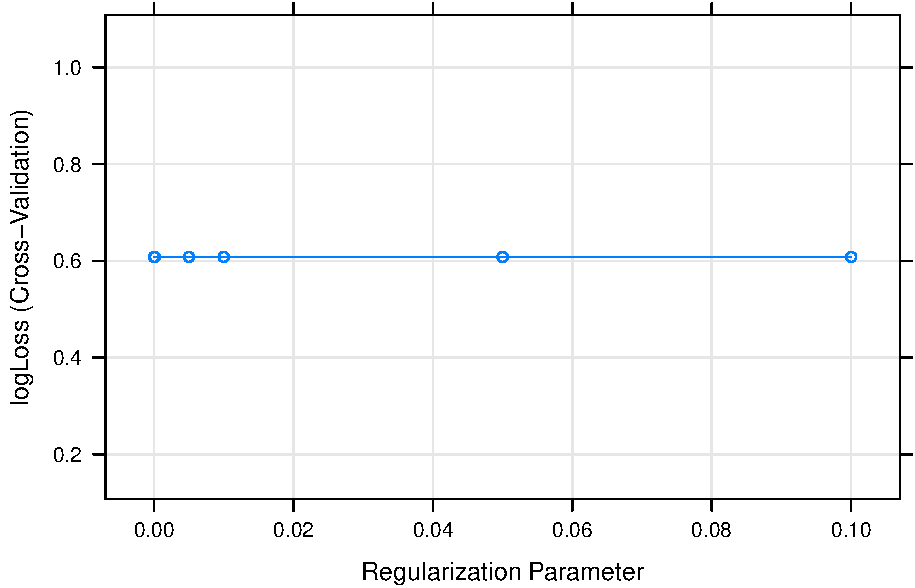
\includegraphics{analysis_files/figure-latex/unnamed-chunk-11-1.pdf}

\begin{verbatim}
##    alpha lambda
## 15     0    0.1
\end{verbatim}

\begin{verbatim}
##          pred_class_12
##            0  1
##   hate    32 82
##   nothate 50 36
\end{verbatim}

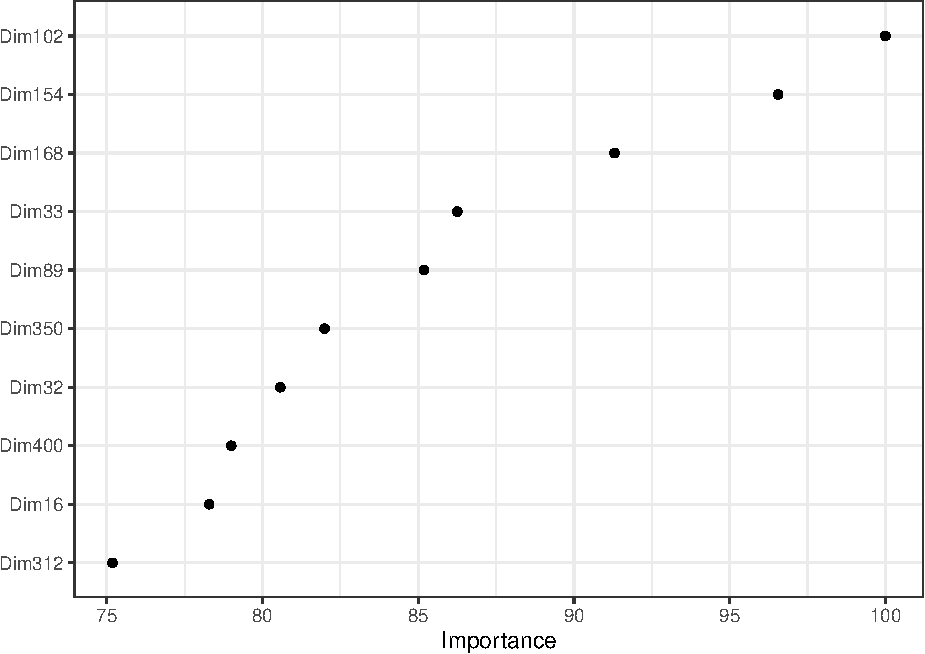
\includegraphics{analysis_files/figure-latex/unnamed-chunk-11-2.pdf}

\begin{verbatim}
## [1] 769
\end{verbatim}

\begin{verbatim}
##              [,1]
## (Intercept) -0.33
## Dim102      -0.15
## Dim154       0.15
## Dim168       0.14
## Dim33       -0.13
## Dim89       -0.13
## Dim350       0.13
## Dim32       -0.12
## Dim400      -0.12
## Dim16        0.12
\end{verbatim}

\hypertarget{logistic-regression-with-lasso-penalty}{%
\subsection{Logistic Regression with Lasso penalty}\label{logistic-regression-with-lasso-penalty}}

\begin{verbatim}
##     alpha lambda
## 1       1  0.016
## 2       1  0.016
## 3       1  0.016
## 4       1  0.016
## 5       1  0.016
## 6       1  0.016
## 7       1  0.016
## 8       1  0.016
## 9       1  0.016
## 10      1  0.016
## 11      1  0.016
## 12      1  0.016
## 13      1  0.016
## 14      1  0.016
## 15      1  0.016
## 16      1  0.016
## 17      1  0.016
## 18      1  0.016
## 19      1  0.016
## 20      1  0.016
## 21      1  0.016
## 22      1  0.016
## 23      1  0.016
## 24      1  0.016
## 25      1  0.016
## 26      1  0.016
## 27      1  0.016
## 28      1  0.016
## 29      1  0.016
## 30      1  0.016
## 31      1  0.016
## 32      1  0.016
## 33      1  0.016
## 34      1  0.016
## 35      1  0.016
## 36      1  0.016
## 37      1  0.016
## 38      1  0.016
## 39      1  0.016
## 40      1  0.016
## 41      1  0.016
## 42      1  0.016
## 43      1  0.016
## 44      1  0.016
## 45      1  0.016
## 46      1  0.016
## 47      1  0.016
## 48      1  0.016
## 49      1  0.016
## 50      1  0.016
## 51      1  0.017
## 52      1  0.017
## 53      1  0.017
## 54      1  0.017
## 55      1  0.017
## 56      1  0.017
## 57      1  0.017
## 58      1  0.017
## 59      1  0.017
## 60      1  0.017
## 61      1  0.017
## 62      1  0.017
## 63      1  0.017
## 64      1  0.017
## 65      1  0.017
## 66      1  0.017
## 67      1  0.017
## 68      1  0.017
## 69      1  0.017
## 70      1  0.017
## 71      1  0.017
## 72      1  0.017
## 73      1  0.017
## 74      1  0.017
## 75      1  0.017
## 76      1  0.017
## 77      1  0.017
## 78      1  0.017
## 79      1  0.017
## 80      1  0.017
## 81      1  0.017
## 82      1  0.017
## 83      1  0.017
## 84      1  0.017
## 85      1  0.017
## 86      1  0.017
## 87      1  0.017
## 88      1  0.017
## 89      1  0.017
## 90      1  0.017
## 91      1  0.017
## 92      1  0.017
## 93      1  0.017
## 94      1  0.017
## 95      1  0.017
## 96      1  0.017
## 97      1  0.017
## 98      1  0.017
## 99      1  0.017
## 100     1  0.017
## 101     1  0.017
## 102     1  0.017
## 103     1  0.017
## 104     1  0.017
## 105     1  0.017
## 106     1  0.017
## 107     1  0.017
## 108     1  0.017
## 109     1  0.017
## 110     1  0.017
## 111     1  0.017
## 112     1  0.017
## 113     1  0.017
## 114     1  0.017
## 115     1  0.017
## 116     1  0.017
## 117     1  0.017
## 118     1  0.017
## 119     1  0.017
## 120     1  0.017
## 121     1  0.017
## 122     1  0.017
## 123     1  0.017
## 124     1  0.017
## 125     1  0.017
## 126     1  0.017
## 127     1  0.017
## 128     1  0.017
## 129     1  0.017
## 130     1  0.017
## 131     1  0.017
## 132     1  0.017
## 133     1  0.017
## 134     1  0.017
## 135     1  0.017
## 136     1  0.017
## 137     1  0.017
## 138     1  0.017
## 139     1  0.017
## 140     1  0.017
## 141     1  0.017
## 142     1  0.017
## 143     1  0.017
## 144     1  0.017
## 145     1  0.017
## 146     1  0.017
## 147     1  0.017
## 148     1  0.017
## 149     1  0.017
## 150     1  0.017
## 151     1  0.018
## 152     1  0.018
## 153     1  0.018
## 154     1  0.018
## 155     1  0.018
## 156     1  0.018
## 157     1  0.018
## 158     1  0.018
## 159     1  0.018
## 160     1  0.018
## 161     1  0.018
## 162     1  0.018
## 163     1  0.018
## 164     1  0.018
## 165     1  0.018
## 166     1  0.018
## 167     1  0.018
## 168     1  0.018
## 169     1  0.018
## 170     1  0.018
## 171     1  0.018
## 172     1  0.018
## 173     1  0.018
## 174     1  0.018
## 175     1  0.018
## 176     1  0.018
## 177     1  0.018
## 178     1  0.018
## 179     1  0.018
## 180     1  0.018
## 181     1  0.018
## 182     1  0.018
## 183     1  0.018
## 184     1  0.018
## 185     1  0.018
## 186     1  0.018
## 187     1  0.018
## 188     1  0.018
## 189     1  0.018
## 190     1  0.018
## 191     1  0.018
## 192     1  0.018
## 193     1  0.018
## 194     1  0.018
## 195     1  0.018
## 196     1  0.018
## 197     1  0.018
## 198     1  0.018
## 199     1  0.018
## 200     1  0.018
## 201     1  0.018
\end{verbatim}

\begin{verbatim}
## glmnet 
## 
## 800 samples
## 768 predictors
##   2 classes: 'hate', 'nothate' 
## 
## Recipe steps: normalize 
## Resampling: Cross-Validated (10 fold) 
## Summary of sample sizes: 720, 720, 720, 720, 720, 720, ... 
## Resampling results across tuning parameters:
## 
##   lambda  logLoss
##   0.016   0.61   
##   0.016   0.61   
##   0.016   0.61   
##   0.016   0.61   
##   0.016   0.61   
##   0.016   0.61   
##   0.016   0.61   
##   0.016   0.61   
##   0.016   0.61   
##   0.016   0.61   
##   0.016   0.61   
##   0.016   0.61   
##   0.016   0.61   
##   0.016   0.61   
##   0.016   0.61   
##   0.016   0.61   
##   0.016   0.61   
##   0.016   0.61   
##   0.016   0.61   
##   0.016   0.61   
##   0.016   0.61   
##   0.016   0.61   
##   0.016   0.61   
##   0.016   0.61   
##   0.016   0.61   
##   0.016   0.61   
##   0.016   0.61   
##   0.016   0.61   
##   0.016   0.61   
##   0.016   0.61   
##   0.016   0.61   
##   0.016   0.61   
##   0.016   0.61   
##   0.016   0.61   
##   0.016   0.61   
##   0.016   0.61   
##   0.016   0.61   
##   0.016   0.61   
##   0.016   0.61   
##   0.016   0.61   
##   0.016   0.61   
##   0.016   0.61   
##   0.016   0.61   
##   0.016   0.61   
##   0.016   0.61   
##   0.016   0.61   
##   0.016   0.61   
##   0.016   0.61   
##   0.016   0.61   
##   0.016   0.61   
##   0.017   0.61   
##   0.017   0.61   
##   0.017   0.61   
##   0.017   0.61   
##   0.017   0.61   
##   0.017   0.61   
##   0.017   0.61   
##   0.017   0.61   
##   0.017   0.61   
##   0.017   0.61   
##   0.017   0.61   
##   0.017   0.61   
##   0.017   0.61   
##   0.017   0.61   
##   0.017   0.61   
##   0.017   0.61   
##   0.017   0.61   
##   0.017   0.61   
##   0.017   0.61   
##   0.017   0.61   
##   0.017   0.61   
##   0.017   0.61   
##   0.017   0.61   
##   0.017   0.61   
##   0.017   0.61   
##   0.017   0.61   
##   0.017   0.61   
##   0.017   0.61   
##   0.017   0.61   
##   0.017   0.61   
##   0.017   0.61   
##   0.017   0.61   
##   0.017   0.61   
##   0.017   0.61   
##   0.017   0.61   
##   0.017   0.61   
##   0.017   0.61   
##   0.017   0.61   
##   0.017   0.61   
##   0.017   0.61   
##   0.017   0.61   
##   0.017   0.61   
##   0.017   0.61   
##   0.017   0.61   
##   0.017   0.61   
##   0.017   0.61   
##   0.017   0.61   
##   0.017   0.61   
##   0.017   0.61   
##   0.017   0.61   
##   0.017   0.61   
##   0.017   0.61   
##   0.017   0.61   
##   0.017   0.61   
##   0.017   0.61   
##   0.017   0.61   
##   0.017   0.61   
##   0.017   0.61   
##   0.017   0.61   
##   0.017   0.61   
##   0.017   0.61   
##   0.017   0.61   
##   0.017   0.61   
##   0.017   0.61   
##   0.017   0.61   
##   0.017   0.61   
##   0.017   0.61   
##   0.017   0.61   
##   0.017   0.61   
##   0.017   0.61   
##   0.017   0.61   
##   0.017   0.61   
##   0.017   0.61   
##   0.017   0.61   
##   0.017   0.61   
##   0.017   0.61   
##   0.017   0.61   
##   0.017   0.61   
##   0.017   0.61   
##   0.017   0.61   
##   0.017   0.61   
##   0.017   0.61   
##   0.017   0.61   
##   0.017   0.61   
##   0.017   0.61   
##   0.017   0.61   
##   0.017   0.61   
##   0.017   0.61   
##   0.017   0.61   
##   0.017   0.61   
##   0.017   0.61   
##   0.017   0.61   
##   0.017   0.61   
##   0.017   0.61   
##   0.017   0.61   
##   0.017   0.61   
##   0.017   0.61   
##   0.017   0.61   
##   0.017   0.61   
##   0.017   0.61   
##   0.018   0.61   
##   0.018   0.61   
##   0.018   0.61   
##   0.018   0.61   
##   0.018   0.61   
##   0.018   0.61   
##   0.018   0.61   
##   0.018   0.61   
##   0.018   0.61   
##   0.018   0.61   
##   0.018   0.61   
##   0.018   0.61   
##   0.018   0.61   
##   0.018   0.61   
##   0.018   0.61   
##   0.018   0.61   
##   0.018   0.61   
##   0.018   0.61   
##   0.018   0.61   
##   0.018   0.61   
##   0.018   0.61   
##   0.018   0.61   
##   0.018   0.61   
##   0.018   0.61   
##   0.018   0.61   
##   0.018   0.61   
##   0.018   0.61   
##   0.018   0.61   
##   0.018   0.61   
##   0.018   0.61   
##   0.018   0.61   
##   0.018   0.61   
##   0.018   0.61   
##   0.018   0.61   
##   0.018   0.61   
##   0.018   0.61   
##   0.018   0.61   
##   0.018   0.61   
##   0.018   0.61   
##   0.018   0.61   
##   0.018   0.61   
##   0.018   0.61   
##   0.018   0.61   
##   0.018   0.61   
##   0.018   0.61   
##   0.018   0.61   
##   0.018   0.61   
##   0.018   0.61   
##   0.018   0.61   
##   0.018   0.61   
##   0.018   0.61   
## 
## Tuning parameter 'alpha' was held constant at a value of 1
## logLoss was used to select the optimal model using the smallest value.
## The final values used for the model were alpha = 1 and lambda = 0.017.
\end{verbatim}

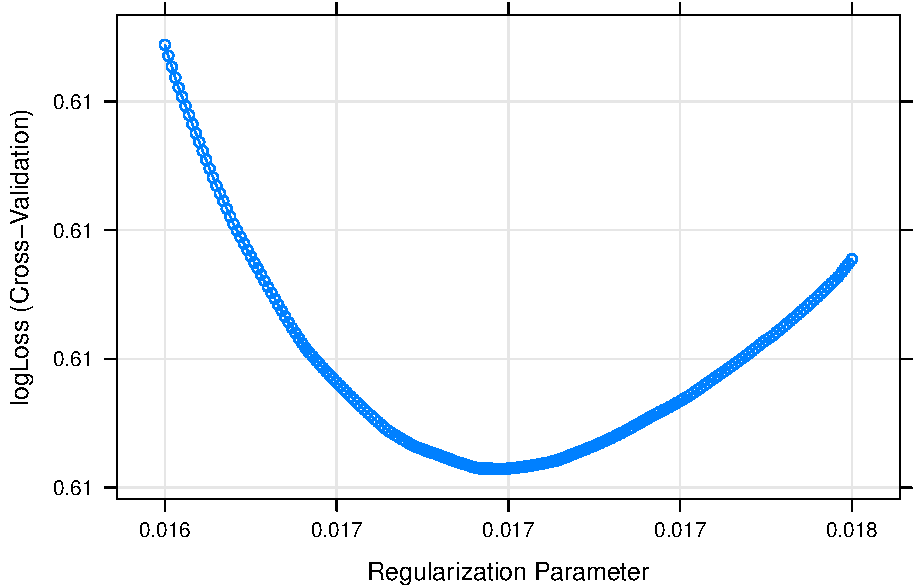
\includegraphics{analysis_files/figure-latex/unnamed-chunk-12-1.pdf}

\begin{verbatim}
##    alpha lambda
## 98     1  0.017
\end{verbatim}

\begin{verbatim}
## [1] 200   2
\end{verbatim}

\begin{verbatim}
##   hate nothate
## 1 0.46    0.54
## 2 0.69    0.31
## 3 0.11    0.89
## 4 0.52    0.48
## 5 0.67    0.33
## 6 0.52    0.48
\end{verbatim}

\begin{verbatim}
## Warning: Unknown or uninitialised column: `hate`.
\end{verbatim}

\begin{verbatim}
##          pred_class_12
##            0  1
##   hate    32 82
##   nothate 50 36
\end{verbatim}

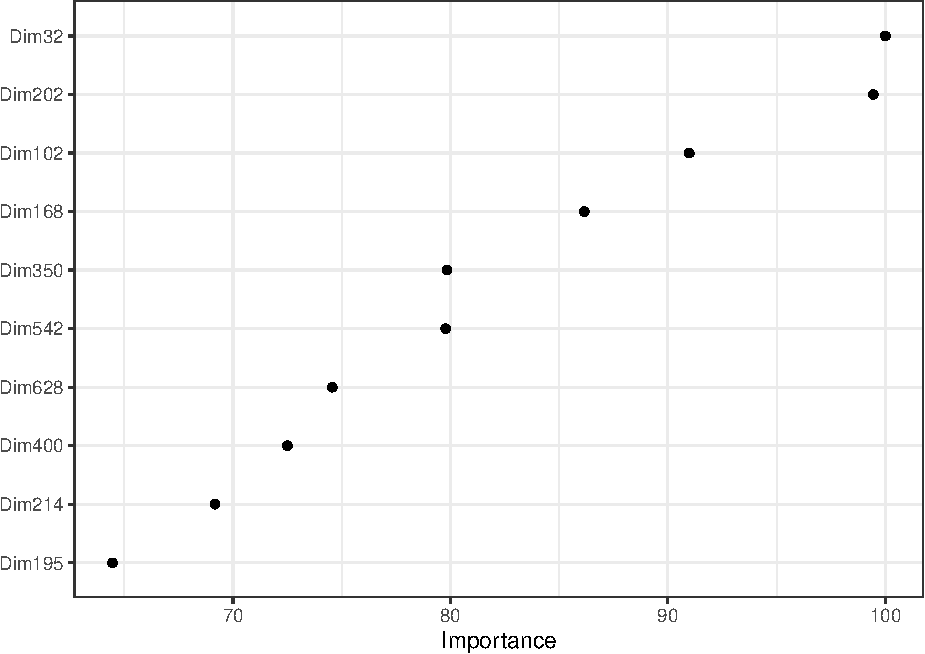
\includegraphics{analysis_files/figure-latex/unnamed-chunk-12-2.pdf}

\begin{verbatim}
##              [,1]
## (Intercept) -0.28
## Dim32       -0.22
## Dim202       0.22
## Dim102      -0.20
## Dim168       0.19
## Dim350       0.18
## Dim542       0.18
## Dim628       0.16
## Dim400      -0.16
## Dim214       0.15
\end{verbatim}

\begin{table}[tbp]

\begin{center}
\begin{threeparttable}

\caption{\label{tab:unnamed-chunk-13}Evaluation metrics for the RoBERTa - Layer 12 model}

\begin{tabular}{llllllll}
\toprule
model & \multicolumn{1}{c}{-LL} & \multicolumn{1}{c}{AUC} & \multicolumn{1}{c}{ACC} & \multicolumn{1}{c}{TPR} & \multicolumn{1}{c}{TNR} & \multicolumn{1}{c}{FPR} & \multicolumn{1}{c}{PRE}\\
\midrule
Logistic Regression & 16.88 & 0.54 & 0.47 & 0.51 & 0.43 & 0.57 & 0.40\\
Logistic Regression with Ridge Penalty & 0.61 & 0.73 & 0.34 & 0.42 & 0.28 & 0.72 & 0.31\\
Logistic Regression with Lasso Penalty & 0.61 & 0.71 & 0.34 & 0.42 & 0.28 & 0.72 & 0.31\\
\bottomrule
\end{tabular}

\end{threeparttable}
\end{center}

\end{table}

\newpage

\hypertarget{references}{%
\section{References}\label{references}}

\begin{verbatim}
## Warning in utils::citation(x[pkg], auto = if (no_citations[pkg]) TRUE else
## NULL): no date field in DESCRIPTION file of package 'recipes'
\end{verbatim}

\begingroup
\setlength{\parindent}{-0.5in}
\setlength{\leftskip}{0.5in}

\hypertarget{refs}{}
\begin{CSLReferences}{1}{0}
\leavevmode\hypertarget{ref-davidson2017automated}{}%
Davidson, T., Warmsley, D., Macy, M., \& Weber, I. (2017). Automated hate speech detection and the problem of offensive language. In \emph{Proceedings of the international AAAI conference on web and social media} (Vol. 11).

\leavevmode\hypertarget{ref-williams2020hate}{}%
Williams, M. L., Burnap, P., Javed, A., Liu, H., \& Ozalp, S. (2020). Hate in the machine: Anti-black and anti-muslim social media posts as predictors of offline racially and religiously aggravated crime. \emph{The British Journal of Criminology}, \emph{60}(1), 93--117.

\end{CSLReferences}

\endgroup


\end{document}
